% Copy the figures directory alongside the main .tex file.
% Requires graphicx and float. Width follows existing Q2 figures (160-mm text block).

% Q4-F1
\begin{figure}[H]
\centering
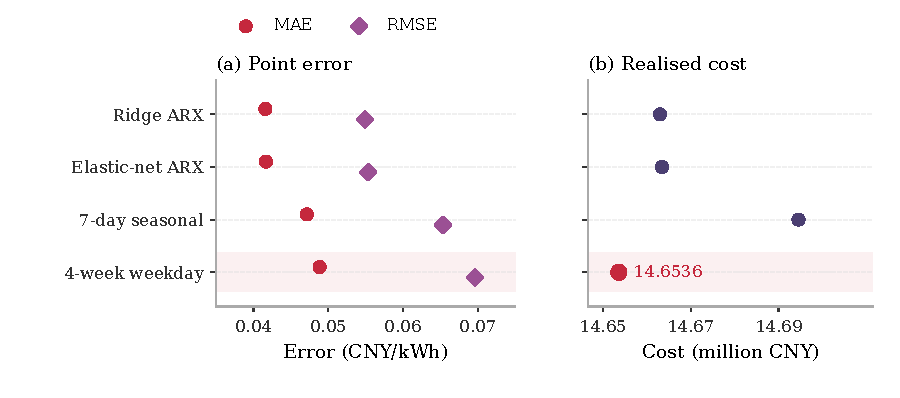
\includegraphics[width=0.96\textwidth]{figures/fig_q4_f1.pdf}
\caption{Forecast error and operational value need not agree. (a) MAE and RMSE of four price forecasters. (b) Realised Q4-2 total expenditure under the same controller; the cost axis is magnified. Ridge ARX minimises point error, whereas the four-week weekday mean gives the lowest cost among the four implementable forecasts (14.6536 million CNY). The selected model is highlighted; the perfect-price diagnostic is excluded.}
\label{fig:q4-f1}
\end{figure}

% Q4-F2
\begin{figure}[H]
\centering
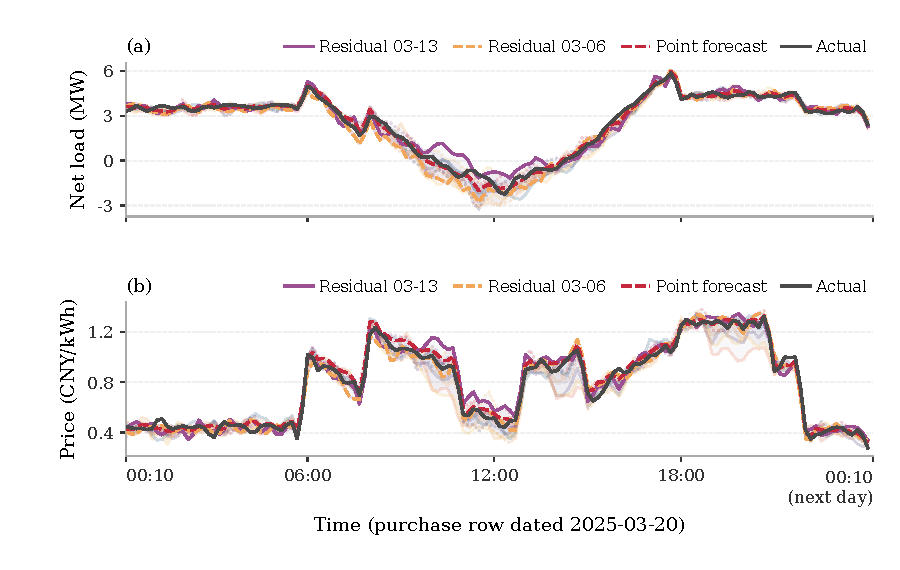
\includegraphics[width=0.96\textwidth]{figures/fig_q4_f2.pdf}
\caption{Paired net-load and price scenarios for 20 March 2025. (a) Net load. (b) Electricity price. All 12 constructed paths are shown faintly; highlighted paths use residuals from 13 March and 6 March in both panels. Nested shading shows the pointwise full range, 10--90\% range and 25--75\% range of these 12 scenarios, not a confidence interval. Actual observations are overlaid only for retrospective evaluation.}
\label{fig:q4-f2}
\end{figure}

% Q4-F3
\begin{figure}[H]
\centering
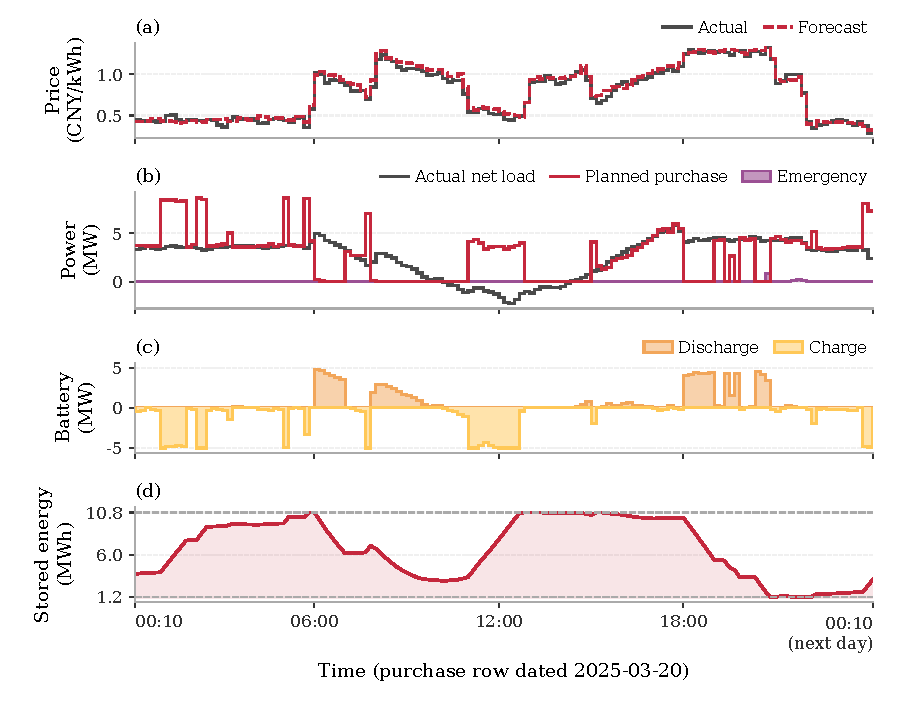
\includegraphics[width=0.96\textwidth]{figures/fig_q4_f3.pdf}
\caption{Q4-2 operation for the purchase row dated 20 March 2025. (a) Actual and forecast price. (b) Actual net load, planned purchase and emergency supply. (c) Discharge (positive) and charge (negative). (d) Realised stored energy, with dashed limits at 1.2 and 10.8 MWh. Purchases and storage respond to the price profile; emergency supply covers residual deficits. Ten-minute purchase energies are converted to average MW.}
\label{fig:q4-f3}
\end{figure}

% Q4-F4
\begin{figure}[H]
\centering
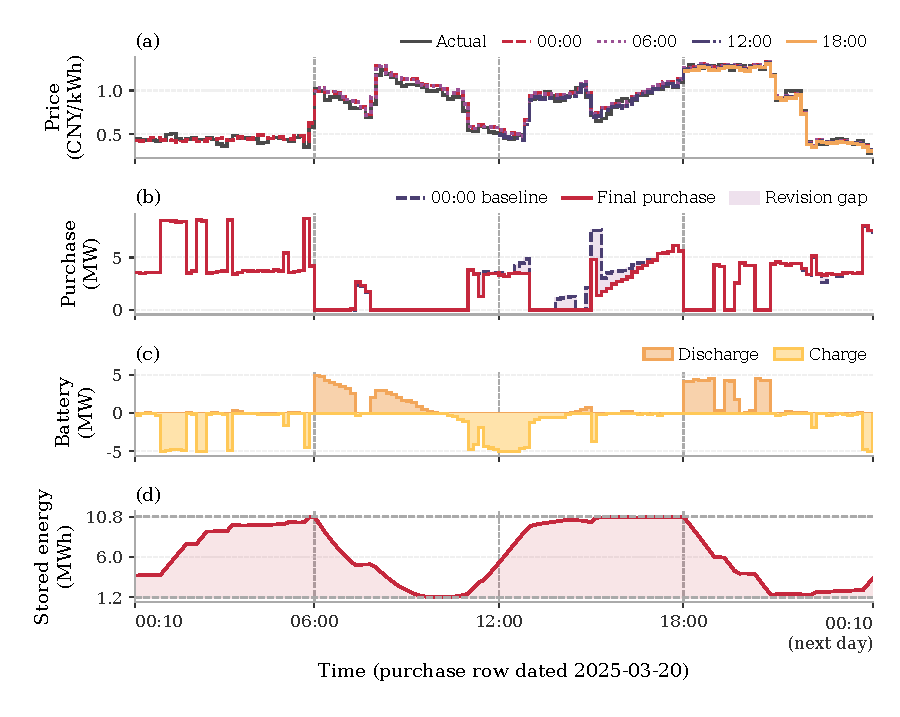
\includegraphics[width=0.96\textwidth]{figures/fig_q4_f4.pdf}
\caption{Q4-3 rolling operation for the purchase row dated 20 March 2025. (a) Actual price and remaining price forecasts issued at 00:00, 06:00, 12:00 and 18:00. (b) Midnight baseline and final executed purchase, with their difference shaded. (c) Realised discharge and charge. (d) Stored energy and its 1.2--10.8 MWh bounds. Vertical lines mark the three intraday issue times. Panel (b) compares the initial and final schedules; it does not display the full sequence of intermediate optimisation tails.}
\label{fig:q4-f4}
\end{figure}

% Q4-F5
\begin{figure}[H]
\centering
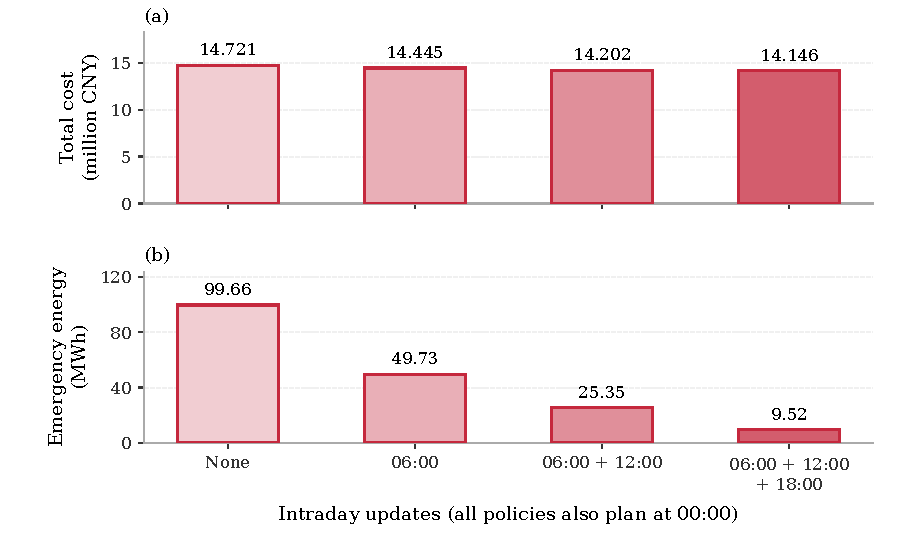
\includegraphics[width=0.96\textwidth]{figures/fig_q4_f5.pdf}
\caption{Value of additional update times within the Q4-3 controller over February--December 2025. (a) Total expenditure. (b) Emergency energy. Both bar axes start at zero. Using all three intraday releases reduces cost from 14.7211 to 14.1463 million CNY (3.905\%) and emergency energy from 99.66 to 9.52 MWh (90.44\%). The four tested nested update subsets show monotone improvement; this is not a claim about every possible subset.}
\label{fig:q4-f5}
\end{figure}

% Q4-F6 -- supplementary
\begin{figure}[H]
\centering
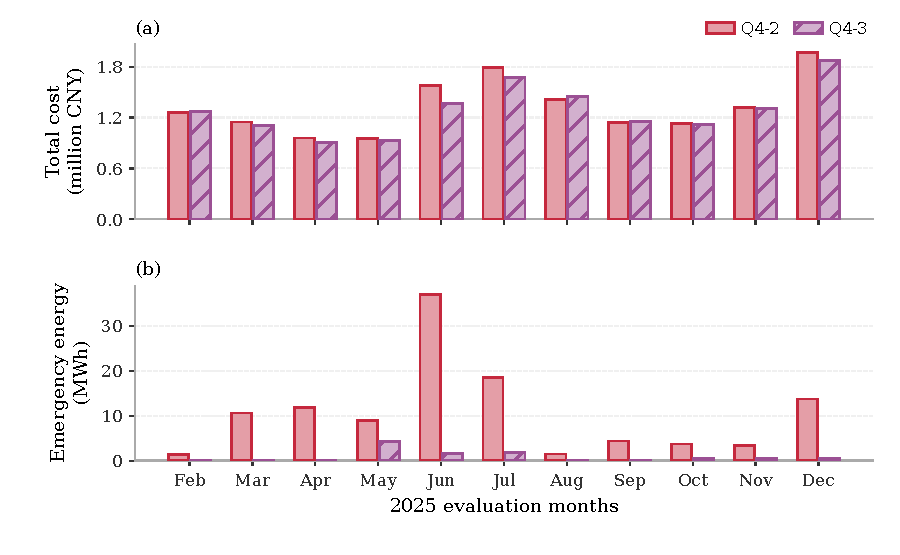
\includegraphics[width=0.96\textwidth]{figures/fig_q4_f6.pdf}
\caption{Monthly outcomes of Q4-2 and Q4-3 during February--December 2025. (a) Total cost. (b) Emergency energy. Q4-3 reduces aggregate expenditure by 507,234.71 CNY (3.461\%), but costs more in February, August and September. Emergency energy is lower in every evaluated month. These are complete-policy comparisons, not an isolated causal effect of adding update times.}
\label{fig:q4-f6}
\end{figure}
